%% Calibration aware neural pre-decoding on one FPGA card
%% Author: Nasir Ali, C-DAC Noida

\documentclass[pdflatex,sn-mathphys-num]{sn-jnl}
\pdfgentounicode=1
\input{glyphtounicode}
\usepackage[T1]{fontenc}
\usepackage{lmodern}
\usepackage{graphicx}
\usepackage{multirow}
\usepackage{amsmath,amssymb,amsfonts}
\usepackage{amsthm}
\usepackage[title]{appendix}
\usepackage{xcolor}
\usepackage{textcomp}
\usepackage{manyfoot}
\usepackage{booktabs}
\usepackage[utf8]{inputenc}
\usepackage{array}
\usepackage{url}
\usepackage{etoolbox}
\AtBeginEnvironment{table}{\small}

\newcommand{\PENDING}[1]{\textcolor{red}{[PENDING: #1]}}
% generated by analysis/summarize.py; do not edit
\newcommand{\NumDevices}{8}
\newcommand{\NumPoints}{108}
\newcommand{\RatioMin}{0.64}
\newcommand{\RatioMax}{1.05}
\newcommand{\NumBetter}{37}
\newcommand{\NumWorse}{3}
\newcommand{\NumMedianPoints}{48}
\newcommand{\PmThreeN}{54}
\newcommand{\PmThreeBetter}{35}
\newcommand{\PmThreeWorse}{4}
\newcommand{\PmThreeMin}{0.85}
\newcommand{\PmThreeMax}{1.17}
\newcommand{\PmFiveN}{54}
\newcommand{\PmFiveBetter}{44}
\newcommand{\PmFiveWorse}{4}
\newcommand{\PmFiveMin}{0.64}
\newcommand{\PmFiveMax}{1.06}
\newcommand{\CorrThreeN}{54}
\newcommand{\CorrThreeBetter}{21}
\newcommand{\CorrThreeWorse}{12}
\newcommand{\CorrThreeMin}{0.73}
\newcommand{\CorrThreeMax}{1.20}
\newcommand{\CorrFiveN}{54}
\newcommand{\CorrFiveBetter}{0}
\newcommand{\CorrFiveWorse}{51}
\newcommand{\CorrFiveMin}{1.07}
\newcommand{\CorrFiveMax}{1.61}
\newcommand{\CorrPmThreeN}{54}
\newcommand{\CorrPmThreeBetter}{25}
\newcommand{\CorrPmThreeWorse}{8}
\newcommand{\CorrPmThreeMin}{0.90}
\newcommand{\CorrPmThreeMax}{1.29}
\newcommand{\CorrPmFiveN}{54}
\newcommand{\CorrPmFiveBetter}{54}
\newcommand{\CorrPmFiveWorse}{0}
\newcommand{\CorrPmFiveMin}{0.50}
\newcommand{\CorrPmFiveMax}{0.87}
\newcommand{\FcCorrThreeN}{54}
\newcommand{\FcCorrThreeBetter}{20}
\newcommand{\FcCorrThreeWorse}{15}
\newcommand{\FcCorrThreeMin}{0.76}
\newcommand{\FcCorrThreeMax}{1.24}
\newcommand{\FcCorrFiveN}{54}
\newcommand{\FcCorrFiveBetter}{0}
\newcommand{\FcCorrFiveWorse}{49}
\newcommand{\FcCorrFiveMin}{0.99}
\newcommand{\FcCorrFiveMax}{1.61}
\newcommand{\MedWeightsMin}{0.97}
\newcommand{\MedWeightsMax}{1.16}
\newcommand{\KingScreenMin}{1.00}
\newcommand{\KingScreenMax}{1.17}
\newcommand{\KingScreenN}{6}
\newcommand{\KingScreenWorse}{5}
\newcommand{\MedWThreeN}{30}
\newcommand{\MedWThreeWorse}{19}
\newcommand{\MedWFiveN}{30}
\newcommand{\MedWFiveWorse}{20}
\newcommand{\TotalShots}{43,200,000}
\newcommand{\LowN}{16}
\newcommand{\LowCorrWorse}{13}
\newcommand{\LowFastBetterCorr}{13}
\newcommand{\BelowPmOne}{3}
\newcommand{\BelowCorrOne}{6}
\newcommand{\BelowFastOne}{3}
\newcommand{\BelowPmHalf}{8}
\newcommand{\BelowCorrHalf}{8}
\newcommand{\BelowFastHalf}{8}
\newcommand{\BelowPmQuarter}{8}
\newcommand{\BelowCorrQuarter}{8}
\newcommand{\BelowFastQuarter}{8}
\newcommand{\ExAachenPm}{4,520}
\newcommand{\ExAachenCorr}{2,823}
\newcommand{\ExAachenFast}{3,347}
\newcommand{\ExAachenFastCorr}{3,306}
\newcommand{\QuantMin}{0.92}
\newcommand{\QuantMax}{1.17}
\newcommand{\QuantBetter}{28}
\newcommand{\QuantWorse}{26}
\newcommand{\QuantN}{108}
\newcommand{\OverlapThree}{50}
\newcommand{\OverlapFive}{68}
\newcommand{\MedianFiveMeanRatio}{0.88}
\newcommand{\BestFiveMeanRatio}{0.83}
\newcommand{\WorstCouplerMin}{11}
\newcommand{\WorstCouplerMax}{130}
\newcommand{\ReadoutOverGateMin}{1.1}
\newcommand{\ReadoutOverGateMax}{5.6}
\newcommand{\CardConfigs}{18}
\newcommand{\CardAllExact}{all}
\newcommand{\CardSameAsCPU}{14}
\newcommand{\CardCompared}{14}
\newcommand{\CardRateDd}{4,201}
\newcommand{\CardLatDd}{1.05}
\newcommand{\CardRateDf}{2,330}
\newcommand{\CardLatDf}{1.50}
\newcommand{\CardRateDh}{1,171}
\newcommand{\CardLatDh}{2.34}
\newcommand{\CardRateDj}{622}
\newcommand{\CardLatDj}{3.84}
\newcommand{\CardRateDl}{360}
\newcommand{\CardLatDl}{6.21}
\newcommand{\CardRateDn}{224}
\newcommand{\CardLatDn}{9.56}
\newcommand{\CpuName}{AMD EPYC 7742 64-Core}
\newcommand{\CpuThreads}{256}
\newcommand{\CpuRateDd}{21,289}
\newcommand{\CpuOverCardDd}{5.1}
\newcommand{\CpuRateDf}{5,595}
\newcommand{\CpuOverCardDf}{2.4}
\newcommand{\CpuRateDh}{2,082}
\newcommand{\CpuOverCardDh}{1.8}
\newcommand{\CpuRateDj}{1,016}
\newcommand{\CpuOverCardDj}{1.6}
\newcommand{\TeachDOneOne}{5.37}
\newcommand{\TeachDTwoKeptOne}{0.181}
\newcommand{\TeachDTwoDiscardOne}{51}
\newcommand{\TeachDThreeOne}{3.33}
\newcommand{\TeachDFiveOne}{1.526}
\newcommand{\TeachDOneHalf}{2.76}
\newcommand{\TeachDTwoKeptHalf}{0.036}
\newcommand{\TeachDTwoDiscardHalf}{30}
\newcommand{\TeachDThreeHalf}{0.95}
\newcommand{\TeachDFiveHalf}{0.213}
\newcommand{\TeachDOneQuarter}{1.40}
\newcommand{\TeachDTwoKeptQuarter}{0.009}
\newcommand{\TeachDTwoDiscardQuarter}{16}
\newcommand{\TeachDThreeQuarter}{0.26}
\newcommand{\TeachDFiveQuarter}{0.028}


\raggedbottom

\begin{document}

\title[Calibration Aware Neural Pre-Decoding on One FPGA]{Neural Pre-Decoding Under Device Calibrated Noise:
IBM Calibration Data, Correlated Matching and Integer Inference on One Alveo U55C}

\author*[1]{\fnm{Nasir} \sur{Ali}}\email{nasirali2607@gmail.com}

\affil*[1]{\orgdiv{Embedded Systems Division},
           \orgname{Centre for Development of Advanced Computing},
           \orgaddress{\city{Noida}, \postcode{201307}, \country{India}}}

\abstract{Neural pre-decoders remove local errors from a surface code syndrome before a matching decoder handles the rest, and
are usually trained and judged on uniform circuit noise. We evaluate NVIDIA's Fast pre-decoder on
memory circuits whose every fault location carries the error rate of a real qubit or coupler, read from IBM
calibration CSV files. Eight IBM devices, three placements of code qubits and three error scales give
\NumPoints{} points at distances 3 and 5, with \TotalShots{} shots. Against plain matching the pre-decoder wins at \PmFiveBetter{} of \PmFiveN{} distance 5 points, with failure ratios down to \PmFiveMin{}. Against
PyMatching with correlated matching, which needs no network, the outcome reverses: the pre-decoder loses at every
distance 5 point (ratios \CorrFiveMin{} to \CorrFiveMax{}), and placing it in front of correlated matching does not
help. It keeps an advantage at distance 3 and low noise, where correlated matching is worse than plain matching. On
strongly uneven qubits the network makes even plain matching worse, by up to \KingScreenMax{} times, while matching
weights from each qubit's calibration beat device medians by up to \MedWeightsMax{} times. The integer network runs
on one Alveo U55C card, bit exact in \CardAllExact{} \CardConfigs{} runs and, in the \CardCompared{} runs with a CPU counterpart,
identical to the CPU integer model in logical failures shot by shot. One card decodes \CardRateDf{} distance 5 windows per second, which a
\CpuThreads{} thread CPU exceeds by \CpuOverCardDf{} times. Calibration files, code and a teaching example for
distances 1 to 5 are released.
}

\keywords{Quantum error correction, Surface code, Neural pre-decoder, Device calibration, Correlated matching,
FPGA, Integer inference, Alveo U55C}

\maketitle

\section{Introduction}\label{sec:intro}

A surface code logical qubit is protected only as long as its syndrome is decoded fast and well
\cite{dennis2002topological,fowler2012surface}. Experiments that operate below the surface code threshold
\cite{google2023scaling,google2025below} have made decoding speed and accuracy questions of system design, and
minimum weight perfect matching, in the Sparse Blossom implementation of PyMatching
\cite{higgott2022pymatching,higgott2025sparse}, is the common reference for both. Neural pre-decoders are one proposal
to improve on it: a small convolutional network looks at a window of syndrome rounds, removes the errors it is sure
of, and leaves a sparser syndrome to the matching decoder
\cite{chamberland2018deep,chamberland2026predecoder}. NVIDIA released two such networks with pretrained weights and
evaluation code \cite{chamberland2026predecoder,nvidia_fast_card,nvidia_ising_code}. In earlier work we implemented them
as an integer kernel on Alveo U55C cards and measured their throughput on four cards \cite{ali2026nodes}.

Those networks were trained, and their published accuracy measured, on circuit noise of one strength at every
location. A device is different. On the IBM devices studied here the two qubit gate error of the worst usable coupler
is \WorstCouplerMin{} to \WorstCouplerMax{} times that of the median one, the median readout error is
\ReadoutOverGateMin{} to \ReadoutOverGateMax{} times the median two qubit gate error, and data qubits idle through
microseconds of ancilla readout with their own $T_1$ and $T_2$. Whether a network trained on uniform noise keeps its
advantage under such noise, and against which matching baseline that advantage should be judged, is the subject of
this paper. A decoder that knows each qubit's rates can also weight its matching graph accordingly
\cite{sivak2024priors}, which raises a second question: how much of any gain comes from the network and how much is
available to matching alone.

We answer both questions with device calibration data, without access to the devices. IBM publishes calibration
snapshots of its devices with qiskit-ibm-runtime \cite{qiskit_ibm_runtime}; we export eight of them to CSV files in the
layout of IBM's own calibration downloads and map every fault location of NVIDIA's memory circuit to the rate of the
qubit or coupler it is assigned to. The pre-decoder then runs unchanged, in floating point and as the integer model
that the FPGA kernel computes, and on one U55C card.

The contributions are:
\begin{itemize}
\item A noise model that keeps the fault locations of NVIDIA's circuit, so the network sees the structure it was
trained on, and sets every location from a calibration CSV: gate errors, readout and preparation errors, and $T_1$ and
$T_2$ decay over the measured durations of gate, readout and reset layers (Section~\ref{sec:methods}).
\item An evaluation over \NumPoints{} points (eight devices, three placements, three error scales, distances 3 and 5)
with paired, shot by shot comparisons against plain matching, matching with device median weights and correlated
matching \cite{fowler2013correlated,paler2023pipelined} (Section~\ref{sec:results}).
\item The finding that correlated matching, with no network, beats the pre-decoder pipeline at every distance 5
point, that the network loses its advantage on strongly uneven qubits, and that calibrated matching weights are worth
up to \MedWeightsMax{} times in logical error on their own.
\item Integer inference of the network on one U55C card, bit exact on every run and identical to the CPU integer
model in every logical failure wherever both were run, with a direct throughput comparison against a \CpuThreads{} thread CPU.
\item A public repository with the calibration files, the experiments and a teaching example that runs codes of
distance 1, 2, 3 and 5 from any calibration CSV on a laptop.
\end{itemize}

\section{Related work}\label{sec:related}

\textbf{Matching and its refinements.} Minimum weight perfect matching on the detector graph of a circuit
\cite{dennis2002topological,fowler2012surface} is the standard surface code decoder, and Sparse Blossom made it fast
enough to decode a million errors per core second \cite{higgott2025sparse}. Union find trades a little accuracy for
almost linear time \cite{delfosse2021unionfind} and has been placed on FPGAs \cite{liyanage2023fpga} and in a real time
decoding system \cite{barber2025decoder}. Matching treats X and Z errors independently, so a Y error, or a two qubit
gate error that flips both, is paid twice. Correlated matching corrects this by reweighting edges after a first pass
\cite{fowler2013correlated,paler2023pipelined}; belief matching does so with belief propagation
\cite{higgott2023belief}. PyMatching exposes correlated matching through a decoding option, which is the strongest
network free baseline used here.

\textbf{Neural decoders and pre-decoders.} Neural decoders for topological codes go back to
\cite{torlai2017neural}; pre-decoders that handle local errors in front of a global decoder to
\cite{chamberland2018deep}, and their hardware cost was studied in \cite{overwater2022neural}. AlphaQubit decoded
experimental data with a transformer trained on simulated and device data \cite{bausch2024alphaqubit}. NVIDIA's Ising
pre-decoders \cite{chamberland2026predecoder} are three dimensional convolutional networks with pretrained weights
\cite{nvidia_fast_card} and open evaluation code \cite{nvidia_ising_code}; their accuracy is reported on uniform circuit
noise against plain matching. Our earlier work \cite{ali2026nodes} implemented them as an integer kernel, in the style
of integer only inference \cite{jacob2018quantization} and FPGA network compilers
\cite{duarte2018hls4ml,umuroglu2017finn}, and measured throughput on four U55C cards. Neither study placed the
networks under device calibrated noise or compared them with correlated matching.

\textbf{Device informed noise and decoder priors.} Google's below threshold experiments decoded with priors fitted to
device data \cite{google2023scaling,google2025below}, and \cite{sivak2024priors} showed that optimizing the priors of
the matching graph lowers the logical error on hardware. Pauli twirled amplitude and phase damping is the usual way to
turn $T_1$ and $T_2$ into circuit noise \cite{ghosh2012decoherence}, and randomized benchmarking
\cite{magesan2011rb} supplies the gate errors that calibration files report. IBM devices use a heavy hexagonal lattice,
on which surface codes need flag qubits or a modified layout \cite{chamberland2020heavyhex}; we do not embed the code
on the lattice (Section~\ref{sec:methods}), but draw its noise from the measured distributions.

\section{Methods}\label{sec:methods}

\subsection{Calibration data}\label{sec:calib}

IBM distributes snapshots of device calibrations with the fake backends of qiskit-ibm-runtime
\cite{qiskit_ibm_runtime} (version 0.50.0, Apache License 2.0). We export \NumDevices{} of them to CSV files in the
column layout of IBM's calibration downloads: per qubit $T_1$, $T_2$, readout assignment error, the probability of
reading 1 after preparing 0, readout length, $\sqrt{X}$ error and gate length, reset length, and per coupler the CZ
or ECR error and gate length. The reader matches column headers by keywords, so a CSV downloaded from IBM's dashboard
loads unchanged; a qubit with any missing value is marked unusable and never placed. Table~\ref{tab:devices} lists
the devices: two Heron r3 snapshots from April 2026, and Heron r2, Heron r1 and Eagle r3 snapshots from February 2025.

\begin{table}[t]
\caption{The eight calibration snapshots: medians over usable qubits and couplers.}\label{tab:devices}
\centering
\setlength{\tabcolsep}{4pt}
% generated by analysis/summarize.py; do not edit
\begin{tabular}{llrrrrrrr}
\toprule
Device & Family & Usable & 2q & 2q error & sx error & Readout & $T_1$ & $T_2$ \\
 & (snapshot) & qubits & gate & (\%) & (\%) & error (\%) & ($\mu$s) & ($\mu$s) \\
\midrule
Aachen & Heron r3 (2026-04) & 156 & CZ & 0.15 & 0.019 & 0.74 & 232 & 255 \\
Kingston & Heron r3 (2026-04) & 155 & CZ & 0.18 & 0.023 & 0.95 & 283 & 144 \\
Marrakesh & Heron r2 (2025-02) & 156 & CZ & 0.32 & 0.023 & 0.95 & 197 & 118 \\
Fez & Heron r2 (2025-02) & 156 & CZ & 0.38 & 0.023 & 0.76 & 145 & 88 \\
Torino & Heron r1 (2025-02) & 132 & CZ & 0.41 & 0.027 & 2.29 & 185 & 141 \\
Sherbrooke & Eagle r3 (2025-02) & 126 & ECR & 0.75 & 0.024 & 1.97 & 279 & 169 \\
Brisbane & Eagle r3 (2025-02) & 127 & ECR & 0.77 & 0.024 & 2.00 & 232 & 150 \\
Kyiv & Eagle r3 (2025-02) & 127 & ECR & 1.15 & 0.025 & 1.27 & 287 & 118 \\
\bottomrule
\end{tabular}

\end{table}

\subsection{Calibrated noise on NVIDIA's memory circuit}\label{sec:noise}

The experiment is a rotated surface code memory of distance $d$ over $d$ rounds in the X or Z basis, built by
NVIDIA's \texttt{MemoryCircuit} with boundary detectors \cite{nvidia_ising_code}: the circuit on which the pre-decoder
was trained and evaluated. NVIDIA's noise model places noise in every round except the last, which is perfect, and
reads the data qubits without noise. We generate the circuit with distinct placeholder probabilities, one per class
of fault location, and replace every placeholder by a channel computed from the calibration of the device qubit or
coupler assigned to that location (Table~\ref{tab:noise}). Detector and observable definitions are untouched, so the
network input, the kernel input and the detector order seen by PyMatching are those of NVIDIA's pipeline.

\begin{table}[t]
\caption{Fault locations of NVIDIA's circuit and their calibrated channels. $r$ is an error per gate from randomized
benchmarking; idle channels use the duration of the layer in which the qubit waits.}\label{tab:noise}
\centering
\begin{tabular}{p{3.2cm}p{8.3cm}}
\toprule
Location & Calibrated channel \\
\midrule
Two qubit gate & two qubit depolarizing with $5r_{2q}/4$ on the pair; one qubit depolarizing with $3r_{sx}$ on the
target (the two Hadamards that turn CZ or ECR into CNOT) \\
Idle during gates & Pauli twirled $T_1$ and $T_2$ decay over the longest coupler of the layer plus two $\sqrt{X}$ gates \\
Idle during readout & the same, over the longest ancilla readout \\
Idle during reset & the same, over the longest ancilla reset \\
Measurement & bit flip with the readout assignment error \\
Preparation & bit flip with half of the probability of reading 1 after preparing 0 \\
\bottomrule
\end{tabular}
\end{table}

For an idle of duration $t$ the Pauli twirl of amplitude and phase damping \cite{ghosh2012decoherence} gives
\begin{equation}
p_x = p_y = \frac{1 - e^{-t/T_1}}{4}, \qquad p_z = \frac{1 - e^{-t/T_2}}{2} - p_x, \label{eq:idle}
\end{equation}
with $T_2$ clipped to $2T_1$. Average gate errors $r$ are converted to depolarizing probabilities with $3r/2$ for one
qubit and $5r/4$ for two qubits. Measurement and preparation flips are told apart by the next operation on the qubit:
a flip followed by a measurement of that qubit is a readout error, any other is a preparation error. The preparation
error takes half of IBM's ``Prob meas1 prep0'' because that quantity contains both the preparation and the readout of
a prepared 0. An error scale $s$ multiplies every probability and every decay rate ($t \to st$ in
Eq.~\ref{eq:idle}), so $s = 0.5$ models a device with half of every error.

\textbf{Placement.} IBM devices are heavy hexagonal and the rotated surface code needs a square grid. We do not embed
the code in the device graph, which would require flag qubits or SWAPs \cite{chamberland2020heavyhex}. Instead, each
code qubit gets a distinct device qubit and each code coupler a distinct device coupler, in one of three modes:
\emph{median} (every location gets the device median, a homogeneous circuit), \emph{best} (the lowest error usable
qubits and couplers) and \emph{screened} (a seeded random draw after removing the worst 10\% of every metric). The
noise is therefore drawn from each device's measured distribution, not a model of running the code on that chip.

\textbf{Experimental points.} Every device is run in the median and best modes at $s = 1$, $0.5$ and $0.25$ and
$d = 3$ and $5$; the two Heron r3 devices are also run with three screened draws at $s = 0.5$. Each point is sampled
with Stim \cite{gidney2021stim}, 200,000 shots per basis, with fixed seeds that make every decoder see the same shots.
The X and Z experiments are pooled, giving \NumPoints{} points of 400,000 shots.

\subsection{Decoders}\label{sec:decoders}

All matching decoders use PyMatching 2.4 \cite{higgott2022pymatching,higgott2025sparse} on the decomposed detector
error model of a circuit:
\begin{description}
\item[PM] plain matching on the calibrated circuit, so every edge has the weight of its own qubits' rates;
\item[PM median] plain matching on the median circuit of the same device, which knows only the averages;
\item[PM-corr] matching with correlations enabled, on the calibrated circuit;
\item[Pre-decoder + PM] NVIDIA's Fast network (four 3D convolutions of width 128, receptive field 9, trained at
$d = 9$ on uniform noise \cite{nvidia_fast_card}) in float32 or as the INT8 integer model, followed by PM on the
residual syndrome, through NVIDIA's evaluation module;
\item[Pre-decoder + PM-corr] the float network followed by PM-corr.
\end{description}
The integer model uses INT8 weights with one scale per output channel, INT8 activations with per layer scales taken
at the 99.99th percentile of 1,024 windows sampled from the same circuit with a different seed, and the GELU as a
lookup table; it is the model the FPGA kernel computes
\cite{ali2026nodes}. A logical failure is a shot whose predicted observable flip differs from the true one. For two
decoders $a$ and $b$ on the same shots we report the ratio of failures and the two sided exact sign test on the shots
where exactly one of them fails; a difference is called significant at $p < 0.05$. The logical error per round is
$\epsilon = \tfrac12\bigl(1 - (1 - 2P)^{1/r}\bigr)$ for a failure probability $P$ over $r$ rounds.

\subsection{One U55C card}\label{sec:card}

The card runs the bitstream of the earlier four card study \cite{ali2026nodes} (SHA256 prefix d399f8d0) on one Alveo
U55C \cite{amd_ds978}: two instances of an integer kernel whose window size, up to $13 \times 13 \times 13$, and
weights are launch arguments. A C++ host on XRT \cite{amd_xrt} streams the test windows of a point to both instances
and reads back one decision bit per site. On the first 4,096 windows of every run, both instances are checked bit
exact against the integer model. The decisions of all 200,000 windows are then passed, as fixed network outputs,
through the same evaluation module and PM, and the logical failures are compared shot by shot with the CPU integer
model. Throughput is measured with both instances busy and two launches in flight, 64 windows per launch, over three
repetitions of about ten seconds; latency is the mean time of a one window launch with one launch in flight, PCIe
transfers and runtime included.
For comparison, the float network is timed in PyTorch on the \CpuName{} host with \CpuThreads{} threads, network
forward pass only, in batches of 4,096 windows.

\subsection{Teaching example}\label{sec:teaching}

Distances 1 and 2 cannot correct errors and are not part of the evaluation. The repository includes a CPU example
that runs them, together with $d = 3$ and $5$, from any calibration CSV with the device medians: $d = 1$ is one
unencoded qubit kept for the duration of the rounds, $d = 2$ discards every shot with a detection event, and $d = 3$
and $5$ are decoded by PM. With the Kingston medians over five rounds it gives logical errors of \TeachDOneOne\% for
the bare qubit, \TeachDTwoKeptOne\% for the kept shots of $d = 2$ (with \TeachDTwoDiscardOne\% of shots discarded),
\TeachDThreeOne\% for $d = 3$ and \TeachDFiveOne\% for $d = 5$ at $s = 1$, and \TeachDFiveQuarter\% for $d = 5$ at
$s = 0.25$. It uses Stim's generated circuits with a simpler noise model and is not compared with the results below.

\section{Results}\label{sec:results}

\subsection{Logical error per round}\label{sec:eps}

Figure~\ref{fig:eps} shows the logical error per round of the homogeneous (median) circuits. At the calibrated rates
($s = 1$) the error per round falls from $d = 3$ to $d = 5$ on \BelowPmOne{} of the \NumDevices{} devices with PM and
on \BelowCorrOne{} with PM-corr; at $s = 0.5$ and $s = 0.25$ it falls on all of them with every decoder. The two
Heron r3 devices are the lowest at every scale, the three Eagle r3 devices the highest. These are properties of the
calibrations under our noise model, not hardware results, but they set the regime: the snapshots place most devices
near or above threshold for this circuit, and the scaled points place them below it.

\begin{figure}[t]
\centering
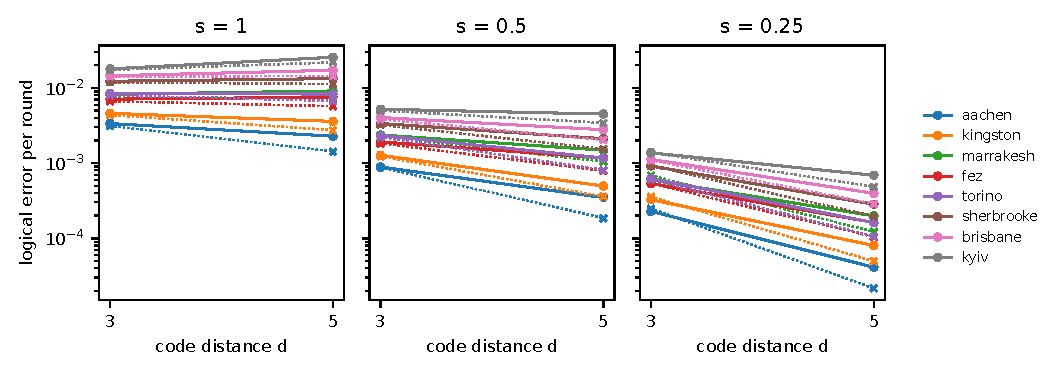
\includegraphics[width=\textwidth]{figures/fig_eps_round.pdf}
\caption{Logical error per round of the median circuits, X and Z pooled. Solid lines: PM; dotted lines: PM-corr.
Panels: error scale $s$.}\label{fig:eps}
\end{figure}

\subsection{The pre-decoder against plain and correlated matching}\label{sec:baselines}

Table~\ref{tab:wins} counts the significant wins and losses of every comparison over all points, and
Fig.~\ref{fig:baselines} shows every failure ratio against the logical error of PM.

\begin{table}[t]
\caption{Paired comparisons over all placements and scales: points where the first decoder fails significantly less
(Better) or more (Worse) often than the second (exact sign test, $p < 0.05$), and the range of failure ratios. The
median weight comparison uses only the best and screened placements, where the two graphs differ.}\label{tab:wins}
\centering
% generated by analysis/summarize.py; do not edit
\begin{tabular}{llrrrr}
\toprule
Comparison & $d$ & Points & Better & Worse & Failure ratio \\
\midrule
INT8 pre-decoder + PM vs PM & 3 & 54 & 35 & 4 & 0.85 to 1.17 \\
INT8 pre-decoder + PM vs PM & 5 & 54 & 44 & 4 & 0.64 to 1.06 \\
INT8 pre-decoder + PM vs PM-corr & 3 & 54 & 21 & 12 & 0.73 to 1.20 \\
INT8 pre-decoder + PM vs PM-corr & 5 & 54 & 0 & 51 & 1.07 to 1.61 \\
float pre-decoder + PM vs PM-corr & 3 & 54 & 17 & 19 & 0.76 to 1.24 \\
float pre-decoder + PM vs PM-corr & 5 & 54 & 0 & 49 & 0.99 to 1.60 \\
float pre-decoder + PM-corr vs PM-corr & 3 & 54 & 20 & 15 & 0.76 to 1.24 \\
float pre-decoder + PM-corr vs PM-corr & 5 & 54 & 0 & 49 & 0.99 to 1.61 \\
PM-corr vs PM & 3 & 54 & 25 & 8 & 0.90 to 1.29 \\
PM-corr vs PM & 5 & 54 & 54 & 0 & 0.50 to 0.87 \\
PM, median weights vs calibrated & 3 & 30 & 0 & 19 & 0.99 to 1.16 \\
PM, median weights vs calibrated & 5 & 30 & 0 & 20 & 0.97 to 1.15 \\
\bottomrule
\end{tabular}

\end{table}

\begin{figure}[t]
\centering
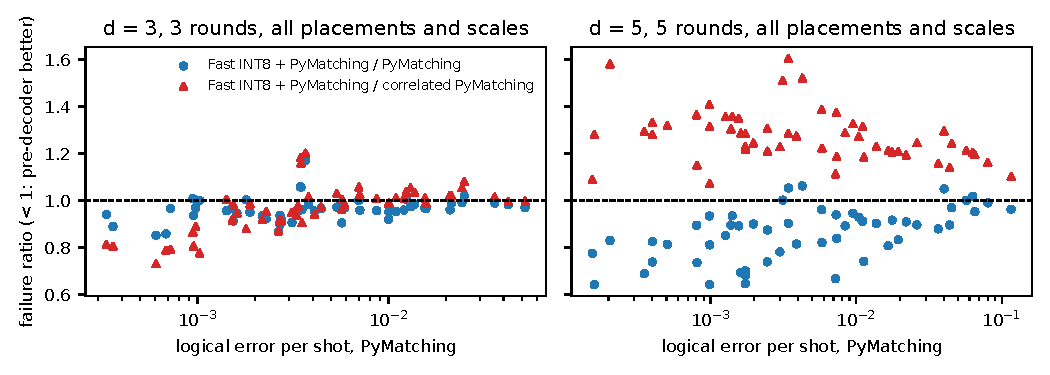
\includegraphics[width=\textwidth]{figures/fig_baselines.pdf}
\caption{Failures of the INT8 pre-decoder followed by PM, divided by the failures of PM (circles) and of PM-corr
(triangles), at every point; X and Z pooled, 400,000 shots per point.}\label{fig:baselines}
\end{figure}

\textbf{Against plain matching} the pre-decoder helps, as NVIDIA reports for uniform noise
\cite{chamberland2026predecoder}: it is significantly better at \PmThreeBetter{} of \PmThreeN{} points at $d = 3$ and
\PmFiveBetter{} of \PmFiveN{} at $d = 5$, with failure ratios down to \PmThreeMin{} and \PmFiveMin{}. The gain is
largest on Aachen, the lowest error device, and smallest on Torino and the Eagle devices, where the ratio approaches
or exceeds 1 at the calibrated rates.

\textbf{Against correlated matching} the result reverses at $d = 5$. PM-corr alone fails less often than the
pre-decoder pipeline at every one of the \CorrFiveN{} points, significantly at \CorrFiveWorse{}, with ratios from
\CorrFiveMin{} to \CorrFiveMax{}. On Aachen at the calibrated rates, for example, PM fails \ExAachenPm{} times in
400,000 shots, the pre-decoder pipeline \ExAachenFast{} and PM-corr \ExAachenCorr{}. PM-corr itself beats PM at every
$d = 5$ point (ratios \CorrPmFiveMin{} to \CorrPmFiveMax{}), and it already corrects most of what the network adds:
of the shots that the pre-decoder pipeline gets right and PM gets wrong, PM-corr gets \OverlapFive{}\% right at
$d = 5$ and \OverlapThree{}\% at $d = 3$. Correlated matching targets faults that flip detectors of both types, such
as Y errors and two qubit gate faults \cite{fowler2013correlated}, which suggests these are a large part of what the
network learned to remove. The float network gives the same picture (Table~\ref{tab:wins}), so this is not an effect of quantization.
Placing the network in front of PM-corr does not help either (\FcCorrFiveBetter{} better,
\FcCorrFiveWorse{} worse at $d = 5$; on Aachen \ExAachenFastCorr{} failures).

At $d = 3$ the picture is mixed. PM-corr is worse than PM at \LowCorrWorse{} of the \LowN{} points at $s = 0.25$, and
there the pre-decoder beats PM-corr significantly at \LowFastBetterCorr{} of them; overall at $d = 3$ the
pre-decoder is better than PM-corr at \CorrThreeBetter{} points and worse at \CorrThreeWorse{}. In this regime,
small codes at low error, the network gains more over plain matching than correlated matching does.

\subsection{Uneven qubits}\label{sec:uneven}

The best placements, whose qubits are all good but differ, behave like the median ones (mean $d = 5$ ratio against
PM \BestFiveMeanRatio{}, against \MedianFiveMeanRatio{} for median). The screened placements draw from most of a
device's spread. On Aachen they still behave like the median ones, but on Kingston the pre-decoder makes plain
matching significantly worse at \KingScreenWorse{} of \KingScreenN{} points, with ratios up to \KingScreenMax{};
these are most of the significant losses in Table~\ref{tab:wins}, the others being Torino and Sherbrooke at the
calibrated rates. A network trained on uniform noise removes errors as if every location were equally likely. When
the rates of the locations differ widely, some of those removals are wrong, while PM, which weights each edge by its
own rate, is not misled in the same way. We read this as a limit of the training distribution rather than of
pre-decoding, which training on calibrated noise could test.

\subsection{Calibrated matching weights}\label{sec:weights}

On the best and screened placements the calibrated circuit and the median circuit differ, and PM can be given
either graph. Figure~\ref{fig:weights} shows the failure ratio of the median graph to the calibrated one. Median
weights are never significantly better, and are significantly worse at \MedWThreeWorse{} of \MedWThreeN{} points at
$d = 3$ and \MedWFiveWorse{} of \MedWFiveN{} at $d = 5$ (Table~\ref{tab:wins}), by up to \MedWeightsMax{} times. This gain needs
no network and no accelerator, only the calibration file, and it is of the same size as the network's gain over PM
at $d = 3$.

\begin{figure}[t]
\centering
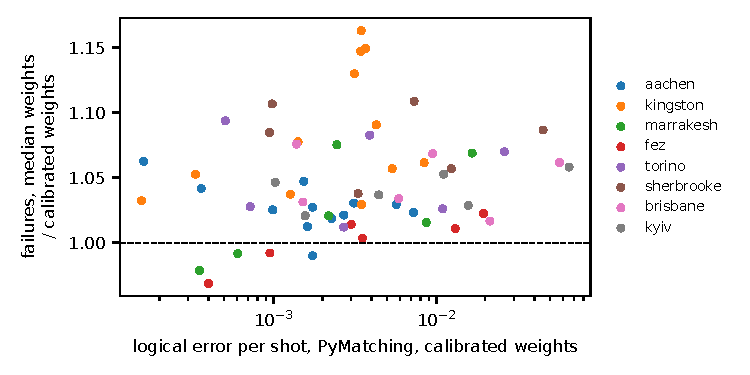
\includegraphics[width=0.75\textwidth]{figures/fig_weights.pdf}
\caption{Failures of PM with the device median graph divided by failures of PM with the calibrated graph, best and
screened placements, against the logical error of the calibrated PM.}\label{fig:weights}
\end{figure}

\subsection{One U55C card}\label{sec:cardres}

Table~\ref{tab:card} lists the \CardConfigs{} card runs. Both kernel instances were bit exact against the integer
model in \CardAllExact{} runs, and in all \CardCompared{} runs that have a CPU integer counterpart the set of shots
on which the card pipeline fails is identical to that of the CPU integer model. The $d = 7$ runs on
Kingston, outside the CPU campaign, show no gain over PM at that distance: the card pipeline fails more often than
PM in three of the four runs.

\begin{table}[t]
\caption{Card runs: logical failures of PM and of the card's INT8 decisions followed by PM on the same 200,000 shots,
and whether the failing shots equal those of the CPU integer model (n/a: no CPU integer run at that
point).}\label{tab:card}
\centering
% generated by analysis/summarize.py; do not edit
\begin{tabular}{lrrlrrrl}
\toprule
Device & Scale & $d$ & Basis & Shots & PM & Card + PM & Same as CPU \\
\midrule
Kingston & 1 & 3 & X & 200,000 & 3,789 & 3,659 & yes \\
Kingston & 1 & 3 & Z & 200,000 & 1,677 & 1,721 & yes \\
Kingston & 1 & 5 & X & 200,000 & 5,257 & 4,847 & yes \\
Kingston & 1 & 5 & Z & 200,000 & 1,820 & 1,637 & yes \\
Kingston & 1 & 7 & X & 200,000 & 5,286 & 5,517 & n/a \\
Kingston & 1 & 7 & Z & 200,000 & 1,355 & 1,409 & n/a \\
Kingston & 0.5 & 3 & X & 200,000 & 1,050 & 1,026 & yes \\
Kingston & 0.5 & 3 & Z & 200,000 & 472 & 472 & yes \\
Kingston & 0.5 & 5 & X & 200,000 & 741 & 658 & yes \\
Kingston & 0.5 & 5 & Z & 200,000 & 246 & 205 & yes \\
Kingston & 0.5 & 7 & X & 200,000 & 432 & 483 & n/a \\
Kingston & 0.5 & 7 & Z & 200,000 & 97 & 88 & n/a \\
Aachen & 1 & 3 & X & 200,000 & 1,898 & 1,757 & yes \\
Aachen & 1 & 3 & Z & 200,000 & 2,105 & 1,925 & yes \\
Aachen & 1 & 5 & X & 200,000 & 2,133 & 1,562 & yes \\
Aachen & 1 & 5 & Z & 200,000 & 2,387 & 1,785 & yes \\
Sherbrooke & 0.5 & 3 & X & 200,000 & 2,284 & 2,164 & yes \\
Sherbrooke & 0.5 & 5 & X & 200,000 & 2,407 & 2,245 & yes \\
\bottomrule
\end{tabular}

\end{table}

Table~\ref{tab:perf} gives throughput and latency. One card decodes \CardRateDd{} windows per second at $d = 3$ and
\CardRateDf{} at $d = 5$; a single window takes \CardLatDd{} and \CardLatDf{} ms through PCIe. The float network on
\CpuThreads{} CPU threads is faster at every distance measured, by \CpuOverCardDd{} times at $d = 3$ and
\CpuOverCardDj{} times at $d = 9$, the gap narrowing as the windows grow. At milliseconds per window, neither is
close to the microsecond syndrome cycle of superconducting devices.

\begin{table}[t]
\caption{Throughput of one card (both kernel instances) and latency of one window, against the float network on the
CPU host (forward pass only, batches of 4,096).}\label{tab:perf}
\centering
% generated by analysis/summarize.py; do not edit
\begin{tabular}{rrrrr}
\toprule
$d$ & Card (windows/s) & One window (ms) & CPU (windows/s) & CPU / card \\
\midrule
3 & 4,201 & 1.05 & 21,289 & 5.1 \\
5 & 2,330 & 1.50 & 5,595 & 2.4 \\
7 & 1,171 & 2.34 & 2,082 & 1.8 \\
9 & 622 & 3.84 & 1,016 & 1.6 \\
11 & 360 & 6.21 & n/a & n/a \\
13 & 224 & 9.56 & n/a & n/a \\
\bottomrule
\end{tabular}

\end{table}

\section{Discussion}\label{sec:discussion}

\textbf{Which baseline.} A pre-decoder is usually judged against the matching decoder it feeds. Our results show why
that is not enough under realistic noise: most of what the network gains over plain matching at $d = 5$ is recovered,
and more, by correlated matching, a decoding option of the same library. The network's advantage at $d = 3$ and low
error is real but small, and it sits where correlated matching is at its weakest. Any claim of a pre-decoder gain
under device noise should therefore name the strongest network free baseline at the same point. Belief matching
\cite{higgott2023belief} and other correlated decoders were not run and might move the bar further.

\textbf{What calibration buys.} The calibration file helps twice. As a noise source it exposes the network to
structure it was not trained on, and on strongly uneven placements the network's uniform prior costs logical
fidelity. As a set of matching weights it improves plain matching by up to \MedWeightsMax{} times with no network at
all, a gain of the same size as the network's own at $d = 3$. The obvious next step, training or fine tuning the
network on calibrated noise, is outside this study; the released noise model produces exactly the training circuits
it would need.

\textbf{What the card shows.} The card reproduces the integer model exactly, shot for shot in logical outcome, so the
FPGA adds no error beyond quantization. Quantization itself is not free under calibrated noise: the integer pipeline
fails \QuantMin{} to \QuantMax{} times as often as the float one, significantly better at \QuantBetter{} and worse at
\QuantWorse{} of \QuantN{} points. The integer scales are fitted to each circuit's own windows; a deployed integer pre-decoder would need the same per
device calibration. As
an accelerator, one card is slower than the \CpuThreads{} thread host for this small network, and at hundreds of
microseconds per round it is far from a microsecond syndrome cycle. The value of the card in this study is as a verified integer
implementation, not as a speedup.

\section{Limitations}\label{sec:limitations}

No circuit was run on IBM hardware. The calibrations set the rates of a simulated circuit; leakage, crosstalk,
measurement induced dephasing beyond $T_2$, drift and correlated errors are not modelled, and gate errors from
randomized benchmarking are treated as depolarizing. The code is not embedded in the heavy hexagonal lattice, so
the results describe noise drawn from each device's distribution, not that device running the code. The snapshots
are single points in time. NVIDIA's network was used as published, trained at $d = 9$ on uniform noise. Throughput
and latency are measured through PCIe with runtime overheads, not in a decoding loop.

\section{Conclusions}\label{sec:conclusions}

We evaluated a published neural pre-decoder on surface code circuits whose noise comes from the calibration files
of eight IBM devices, over \NumPoints{} points and \TotalShots{} shots, and ran its integer form on one Alveo U55C.
Against plain matching the pre-decoder helps at most points, as reported for uniform noise. Against correlated
matching, which needs no network, it loses at every distance 5 point, and putting it in front of correlated matching
does not help; it keeps an edge only for small codes at low error. On strongly uneven qubits the network trained on
uniform noise makes plain matching worse, while matching weights from the calibration file improve it. The card
computes the integer network exactly, with logical outcomes identical to the CPU model wherever both were run, but
more slowly than a large
CPU. A pre-decoder for real devices will need to be trained on device like noise and judged against correlated
matching; the released calibration files, noise model and experiments are a basis for both.


\backmatter

\bmhead{Acknowledgments}
This work was funded by the Ministry of Electronics and Information Technology (MeitY), Government of India. The
research was conducted at the C-DAC Noida Centre under the supervision of Mr. Abhishek Tiwari, Scientist F, Embedded
Systems Division, C-DAC Noida. We thank NVIDIA for releasing the Ising pre-decoders with their evaluation code and
pretrained weights, IBM for publishing device calibration snapshots with qiskit-ibm-runtime, and the developers of
Stim and PyMatching, on which the evaluation of this work depends.

\section*{Declarations}

\textbf{Funding.} This work was funded by the Ministry of Electronics and Information Technology (MeitY), Government of
India.

\textbf{Conflict of interest.} The author declares no competing interests.

\textbf{Ethics approval and consent to participate.} Not applicable.

\textbf{Consent for publication.} Not applicable.

\textbf{Data availability.} The calibration files, the per shot failure records of every decoder at every
experimental point, the card measurement records and the scripts that generate every table and figure from them are
available from the corresponding author on reasonable request. The calibration snapshots are distributed with
qiskit-ibm-runtime under the Apache License 2.0 \cite{qiskit_ibm_runtime}; the pretrained network is available from
NVIDIA under the NVIDIA Open Model License \cite{nvidia_fast_card}.

\textbf{Author contribution.} N.~Ali designed the calibration driven noise model and the experiments, implemented the
evaluation harness and the card runtime, carried out the measurements and wrote the manuscript.

\bibliography{references}

\end{document}
